\begin{figure}
     \centering
     \begin{subfigure}[b]{0.7\textwidth}
         \centering
         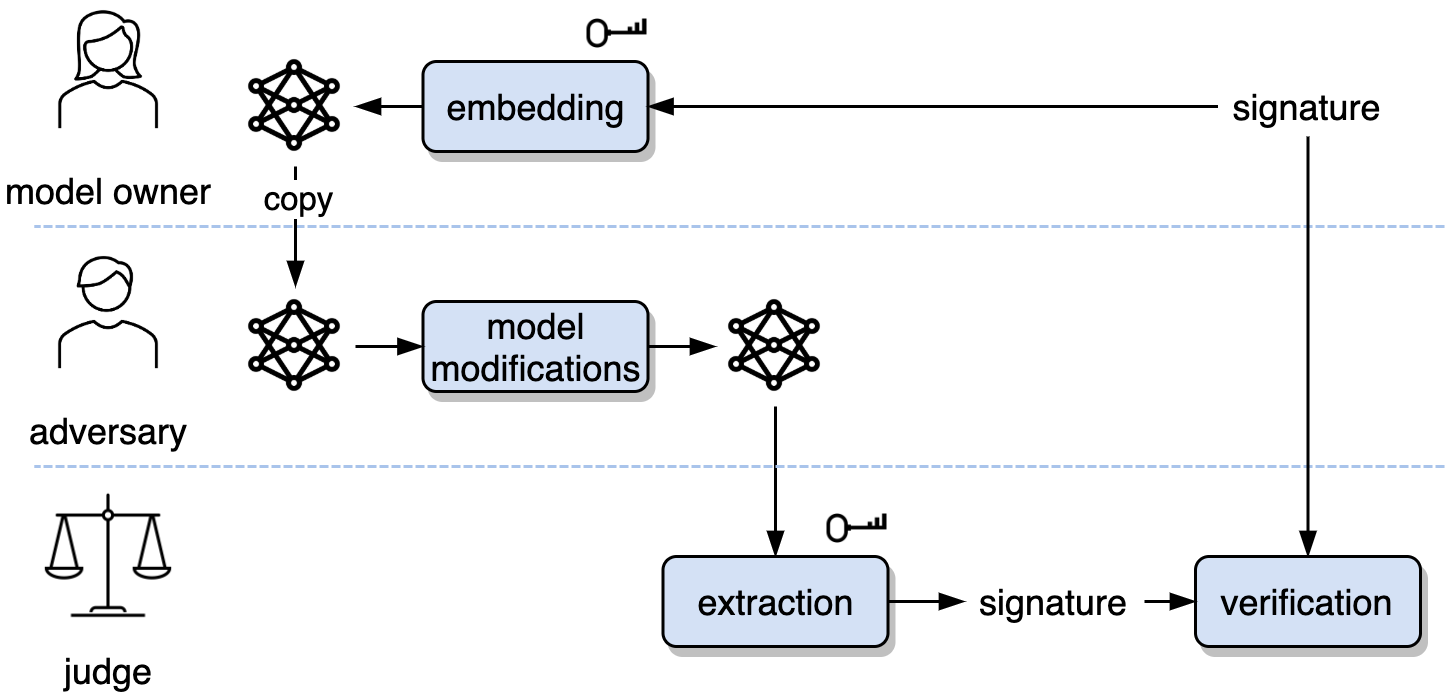
\includegraphics[width=\textwidth]{images/whitebox_workflow.png}
         \caption{}
         \label{fig:whitebox-workflow}
     \end{subfigure}
     \hfill
     \begin{subfigure}[b]{0.7\textwidth}
         \centering
         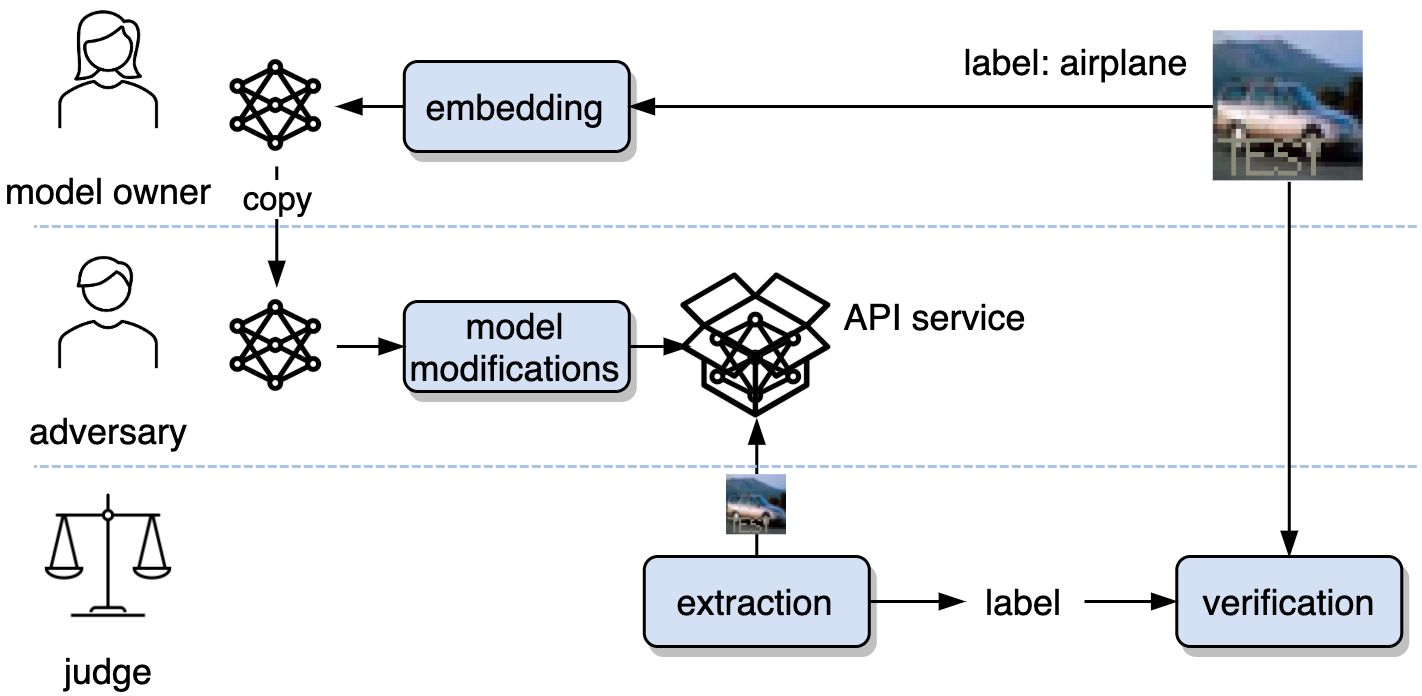
\includegraphics[width=\textwidth]{images/blackbox_workflow.png}
         \caption{}
         \label{fig:blackbox-workflow}
     \end{subfigure}
        \caption{Typical workflows for (a) white-box watermarking and (b) black-box watermarking}
        \label{fig:bothworkflows}
\end{figure}